\documentclass{article}

% Package necessari
\usepackage[a4paper]{geometry}
\usepackage[utf8]{inputenc}
\usepackage[italian]{babel}
\usepackage[T1]{fontenc}
\usepackage[font={small,sl}]{caption}
\usepackage[font={small,sl}]{subcaption}
\usepackage{graphicx}
\usepackage[usenames, table, dvipsnames]{xcolor}
\usepackage{hyperref}
\usepackage[most]{tcolorbox}
\usepackage[section]{placeins}
\usepackage{soulutf8}
\usepackage{listings}
% \usepackage{hhline}

% Titolo del documento
\title{\small Relazione del progetto di Sistemi Operativi Avanzati \\
\Huge \textbf{Multi-flow Device File}}

% Autore del documento
\author{Simone Tiberi (M. 0299908)\\%
(email: \texttt{\href{mailto:simone.tiberi.98@gmail.com}{simone.tiberi.98@gmail.com}})}

% Data del documento
\date{\today}

% Impostazione delle lunghezze di alcuni elementi del documento
\setlength{\parskip}{1em}
\setlength{\parindent}{0em}

% Impostazioni del package hyperref
\hypersetup{
        colorlinks=true,
        linktocpage=true,
        linkcolor=blue,
        urlcolor=blue,
        pdftitle={Relazione progetto SOA},
        pdfauthor={Simone Tiberi},
}

\lstset{
	language=C,
	frame=shadowbox,
	rulesepcolor=\color{gray!50},
	basicstyle=\ttfamily\small,
	keywordstyle=\color{purple}\bfseries\small,
	stringstyle=\color{ForestGreen}\small,
	commentstyle=\color{blue}\small,
	numbers=left,
	numberstyle=\small\color{gray},
	numbersep=5pt,
	tabsize=2,
	showtabs=false,
	showspaces=false,
	showstringspaces=false,
	escapechar=|,
	captionpos=b,
	breaklines=true,
	keepspaces=true
}

\renewcommand{\lstlistingname}{Listato}
\graphicspath{ {./figs/} }

\newtcolorbox{custombox}[1]{
        colframe = blue!25,
        colback  = blue!10,
        coltitle = blue!20!black,
        title    = #1,
        breakable,
        enhanced,
}

% Tabelle
\renewcommand{\arraystretch}{1.5}
\setlength{\arrayrulewidth}{0.1em}

\begin{document}
\maketitle

\section*{Specifica del progetto (traduzione)}
La specifica richiede l'implementazione di un device driver per Linux per la gestione di flussi di dati a due livelli di priorità. Attraverso una sessione aperta verso un dispositivo, un thread può leggere/scrivere dati in modo tale che:
\begin{itemize}
        \item la consegna dei dati segua una politica \textbf{FIFO} (\textbf{F}irst-\textbf{I}n-\textbf{F}irst-\textbf{O}ut),
        \item non appena letti i dati \textbf{scompaiano} dal flusso,
        \item la scrittura sul flusso ad alta priorità sia \textbf{sincrona},
        \item la scrittura sul flusso a bassa priorità sia \textbf{asincrona}, basata su deferred work, \ul{mantenendo comunque la sincronia nella notifica dell'esito dell'operazione} (in conformità all'interfaccia della \texttt{write}),
        \item la scrittura sia sempre eseguita in modo sincrono,
        \item il driver supporti al più \textbf{128} devices associati al corrispettivo minor number.
\end{itemize}

Il device driver deve implementare il supporto all'operazione \texttt{ioctl} al fine di gestire le sessioni di I/O e permettere:
\begin{itemize}
        \item di impostare il livello di priorità (\texttt{HIGH} or \texttt{LOW}) per le operazioni,
        \item di scegliere se effettuare letture e/o scritture in modo bloccante o meno,
        \item di impostare un timeout per regolare il risveglio in caso di richieste bloccanti
\end{itemize}

Inoltre è richiesto di implementare un meccanismo per abilitare o disabilitare i dispositivi in termini di minor numbers, basato sui parametri del modulo. Nel caso in cui un dispositivo sia disabilitato, ogni tentativo di apertura di nuova sessione deve fallire, ma devono comunque continuare ad essere gestite quelle aperte in precedenza.

Altri parametri addizionali esposti tramite VFS devono fornire un'immagine dello stato corrente dei device in termini di:
\begin{itemize}
        \item stato corrente (\texttt{ENABLED} o \texttt{DISABLED}),
        \item numero di byte correntemente presenti nei due flussi,
        \item numero di thread correntemente in attesa nei due flussi
\end{itemize}

\section*{Struttura del repository}
La realizzazione della specifica è stata organizzata all'interno del repository nelle seguenti cartelle:
\begin{itemize}
        \item nella radice è presente uno script \texttt{bash} per la creazione di nodi di I/O pilotabili con il driver sviluppato,
        \item in \texttt{KERNEL\_MODULE/} è contenuto il codice effettivo del driver,
        \item in \texttt{USER\_LIB/} è contenuta una libreria utente per facilitare l'interfacciamento utente con i nodi di I/O associati al driver sviluppato,
        \item in \texttt{SAMPLES/} sono presenti una semplice demo e un file contenente diversi test cases
\end{itemize}

\section*{Driver per la gestione dei dispositivi multi-flusso}
\begin{figure}[htbp]
        \centering
        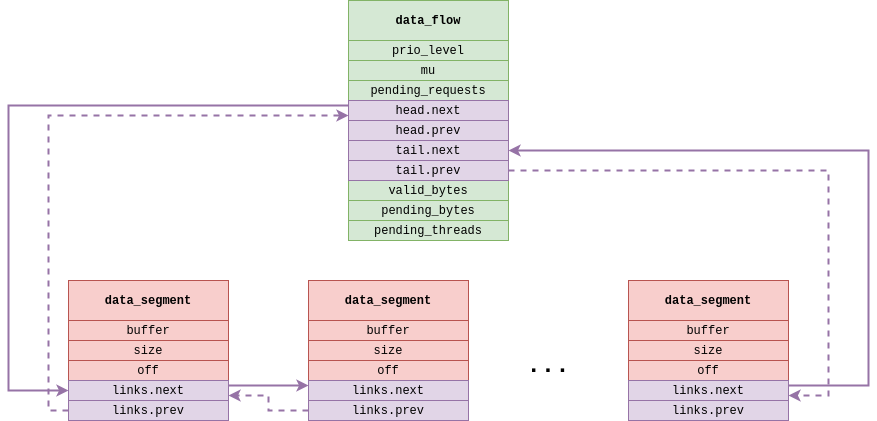
\includegraphics[width=.8\textwidth]{data}
        \caption{Gestione dei dati all'interno dei vari devices}
        \label{fig:data}
\end{figure}

In figura \ref{fig:data} è riportato uno schema dell'architettura adottata all'interno della soluzione proposta per la gestione dei dati. Una delle strutture adottate per la realizzazione dell'implementazione è la \texttt{data\_flow}, la quale rappresenta il singolo flusso di dati associato ad un device.

In essa sono presenti:
\begin{itemize}
        \item il livello di priorità (\texttt{HIGH\_PRIO} o \texttt{LOW\_PRIO}), la cui utilità è descritta in seguito,
        \item il mutex per garantire l'atomicità nell'aggiornamento delle strutture dati necessarie alla gestione del flusso di dati,
        \item la wait queue dove i thread possono attendere nel caso in cui le loro richieste bloccanti non sono al momento soddisfacibili,
        \item la testa e la coda di una lista collegata per l'effettiva memorizzazione dei dati, il cui meccanismo di collegamento è esemplificato in figura \ref{fig:data},
        \item il numero di byte \textit{validi}, ovvero scritti ma non ancora letti,
        \item il numero di byte \textit{pendenti}, ovvero accettati come deferred work ma non ancora effettivamente scritti nel flusso,
        \item il numero di thread in attesa della disponibilità di dati da leggere o di spazio utilizzabile in scrittura.
\end{itemize}

Un ulteriore struttura presente in figura \ref{fig:data} è la \texttt{data\_segment}, la quale rappresenta il chunk di dati scritto sul flusso da una singola operazione di scrittura. Per questo motivo al suo interno sono presenti:
\begin{itemize}
        \item il buffer effettivo in cui memorizzare i dati scritti,
        \item la dimensione complessiva dei dati scritti dall'operazione,
        \item l'offset a cui iniziare a leggere i dati,
        \item una coppia di pointers (\texttt{struct list\_head}) per il collegamento con gli altri chunks.
\end{itemize}

Dalla specifica si evince come ogni device $i$ (con $0\leq i \leq 127$) debba supportare due flussi di dati associati a priorità distinte e che la selezione del livello su cui effettuare le operazioni sia \textbf{per sessione}, per cui in figura \ref{fig:get_active_flow} è riportato lo schema della soluzione scelta per implementare questa meccanica.

\begin{figure}[htbp]
        \centering
        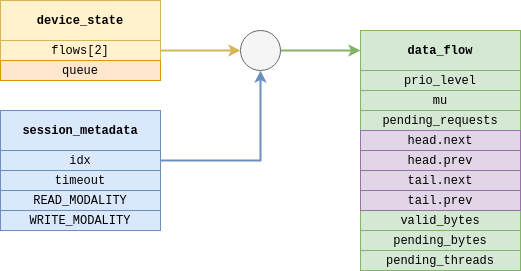
\includegraphics[width=.8\textwidth]{get_active_flow}
        \caption{Come reperire il flusso attualmente attivo a partire dalla sessione}
        \label{fig:get_active_flow}
\end{figure}

In particolare in essa sono compaiono altre due nuove strutture:
\begin{itemize}
        \item la \texttt{device\_state} in cui sono contenuti i metadati associati al dispositivo, ovvero:
                \begin{itemize}
                        \item il vettore dei due flussi di dati associati al dispositivo,
                        \item la work queue in cui accodare le scritture \texttt{LOW\_PRIO} che debbono essere gestite in modo deferred;
                \end{itemize}
        \item la \texttt{session\_metadata} che raccoglie al suo interno il set minimale di informazioni necessarie per la gestione della sessione aperta verso un device, quali:
                \begin{itemize}
                        \item l'indice per spiazzarsi all'interno dell'array di flussi contenuto all'interno della struttura \texttt{device\_state},
                        \item il timeout da utilizzare nel caso in cui si deve attendere per dati da leggere o spazio utilizzabile in scrittura,
                        \item le modalità, bloccanti o meno, di lettura e scrittura.
                \end{itemize}
\end{itemize}

È opportuno osservare che tutti i campi della struttura \texttt{session\_metadata} vengono acceduti atomicamente, o perché definiti come \texttt{atomic[\_long]\_t}, o perché sono singoli bit.

In definitiva dunque l'iter per reperire il riferimento al flusso corrente adottato in tutta l'implementazione è il seguente:
\begin{enumerate}
        \item si accede all'array globale \texttt{struct device\_state devs[MINORS]} utilizzando il minor number come indice, reperito in modalità differenti a seconda della versione del kernel Linux in esercizio,
        \item si preleva dalla sessione l'indice di priorità attualmente configurato e lo si usa per spiazzarsi all'interno dell'array \texttt{flows}.
\end{enumerate}

\subsection*{File operation: \texttt{open}}
La \texttt{mfdf\_open}, ovvero l'implementazione all'interno del driver dell'operazione di apertura è molto semplice e si limita a:
\begin{itemize}
        \item verificare se il dispositivo è correntemente abilitato, ed in caso contrario restituire il codice d'errore \texttt{EAGAIN} al chiamante,
        \item allocare, mediante SLAB allocator, una \texttt{session\_metadata} descritta poc'anzi e collegarla alla \texttt{struct file} sfruttando l'apposito pointer generico \texttt{private\_data},
        \item inizializzare i campi della sessione a valori di default (e.g. flusso attivo: \texttt{LOW\_PRIO}).
\end{itemize}

\subsection*{File operation: \texttt{release}}
La \texttt{mfdf\_release}, ovvero l'implementazione all'interno del driver dell'operazione di rilascio, essendo duale dell'apertura si limita a liberare il buffer allocato per la memorizzazione dei metadati relativi alla sessione.

\end{document}
